\documentclass[../../../thesis.tex]{subfiles}
\begin{document}
    \subsubsection{Pipeline}
    I channel possono essere usati per connettere le goroutine insieme cosicché l'output di uno è l'input dell'altro.
    Questi è detto \textit{pipeline}.
    Il seguente programma consiste di tre goroutine connesse da due channel, come mostrato schematicamente in figura.
    \center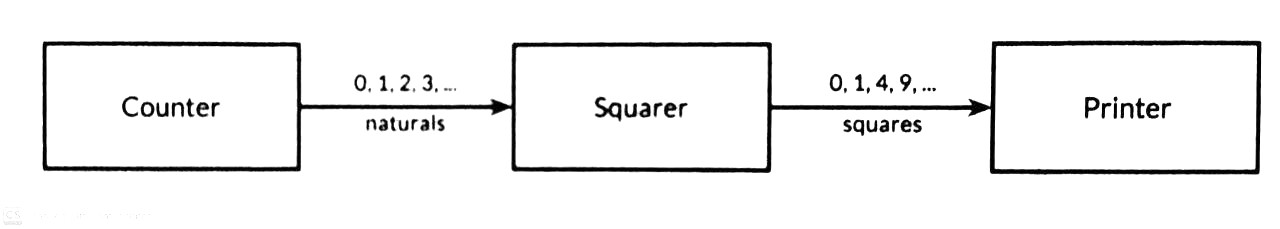
\includegraphics[scale = 0.25]{figure-8.1}

    \justifying\noindent La prima goroutine, \textit{counter}, genera gli interi 0, 1, 2, \ldots, e li invia su un channel alla seconda goroutine, \textit{squarer}, che riceve ogni valore, lo eleva al quadrato, e invia il risultato su un altro channel alla terza goroutine, \textit{printer}, che riceve i valori e li stampa.
    Per chiarezza di quest'esempio, si è intenzionalmente scelto una funzione davvero semplice per spiegare il funzionamento della pipeline.
    \begin{lstlisting}[frame = single,label={lst:lstlisting7-4-2.1}]
func main() {
    naturals := make(chan int)
    squares := make(chan int)

    // Counter
    go func() {
        for x := 0; ; x++ {
            naturals <- x
        }
    }()

    // Squarer
    go func() {
        for {
            x := <-naturals
            squares <- x * x
        }
    }()

    // Printer (nella main goroutine)
    for {
        fmt.Println(<-squares)
    }
}
    \end{lstlisting}
    Se il mittente conosce che non ci sono più valori da inviare sul channel, è bene comunicarlo alla goroutine destinataria così da non farlo attendere.
    Questo è realizzato con la \textit{chiusura} del channel con la funzione built-in \verb"close":
    \begin{lstlisting}[frame = single,label={lst:lstlisting7-4-2.2}]
close(naturals)
    \end{lstlisting}
    Dopo che un channel è stato chiuso, qualunque altra operazione di send restituirà un panic.
    Dopo che il channel chiuso sia stato \textit{svuotato}, ovvero dopo che l'ultimo elemento inviato sia stato recepito, tutte le successive operazioni di receive verranno risolte restituendo un valore zero per il tipo elementare del channel.
    Chiudendo il channel \verb"naturals" si causerà al ciclo di squarer di ricevere uno stream senza fine di valori zero, e di inviare tali valori al printer.
    \hfill \vspace{12pt}

    Non esiste un modo diretto per capire se un channel è stato chiuso, ma esiste una variante dell'operazione di receive che produce due risultati: l'elemento ricevuto dal channel più un valore booleano, denominato per convenzione \verb"ok", che è \verb"true" nel caso di un'operazione di receive completata con successo e \verb"false" nel caso di un'operazione di receive su un channel chiuso e svuotato.
    Usando questa funzionalità, il ciclo di squarer può essere modificato così da interromperlo quando il channel \verb"naturals" è svuotato e chiudere a cascata il channel \verb"squares".
    \begin{lstlisting}[frame = single,label={lst:lstlisting7-4-2.3}]
// Squarer
go func() {
    for {
        x, ok := <-naturals
        if !ok {
            break // il channel %*\textit{è}*) stato chiuso e svuotato
        }
        squares <- x * x
    }
    close(squares)
}()
    \end{lstlisting}
    Il linguaggio permette di usare un ciclo \verb"range" per iterare anche su un channel.
    Questo è sintatticamente più conveniente per ricevere tutti i valori inviati su un channel e terminare il ciclo dopo l'ultimo.
    \begin{lstlisting}[frame = single,label={lst:lstlisting7-4-2.4}]
func main() {
    naturals := make(chan int)
    squares := make(chan int)

    // Counter
    go func() {
        for x := 0; x < 100; x++ {
            naturals <- x
        }
        close(naturals)
    }()

    // Squarer
    go func() {
        for x := range naturals {
            squares <- x * x
        }
        close(squares)
    }()

    // Printer (nella main goroutine)
    for x := range squares {
        fmt.Println(x)
    }
}
    \end{lstlisting}
    Non è sempre necessario chiudere un channel, lo è nel momento in cui è importante avvisare la goroutine destinaria che tutti i valori sono stati inviati, altrimenti può anche essere tralasciato perché il garbage collector si occuperà di determinare quando un channel è diventato irraggiungibile e quindi riciclarlo anche se non chiuso. (Questo discorso non vale per i file;
    i file devono sempre essere chiusi tramite chiamata al metodo \verb"Close").
\end{document}